This chapter presents the results of the data experiments introduced and explained in chapter ??.

\section{Complete pooling, No pooling, Partial pooling}

\begin{figure}
	\subfloat[NHL]{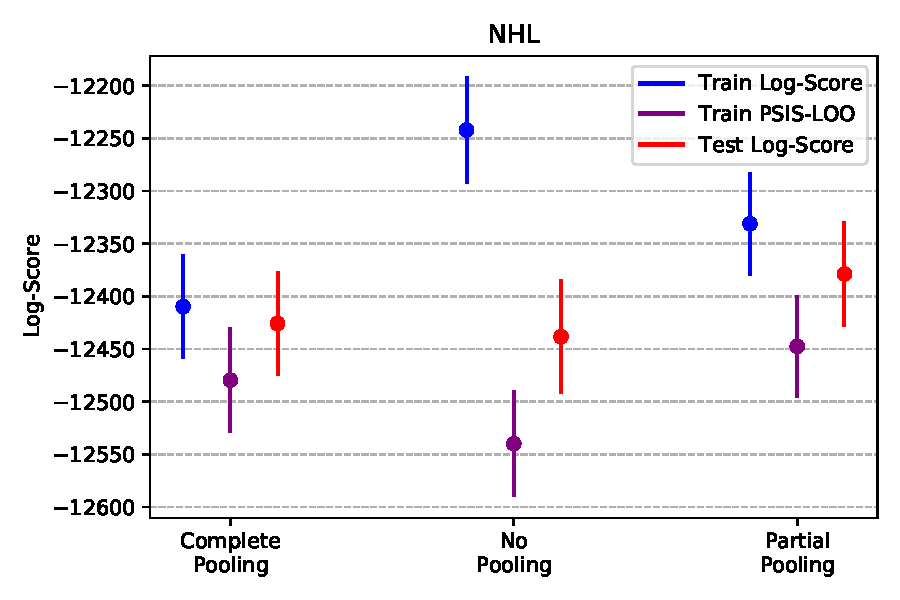
\includegraphics[width=0.5\textwidth]{figures/logscore_NHL.pdf}} 
	\subfloat[NBA]{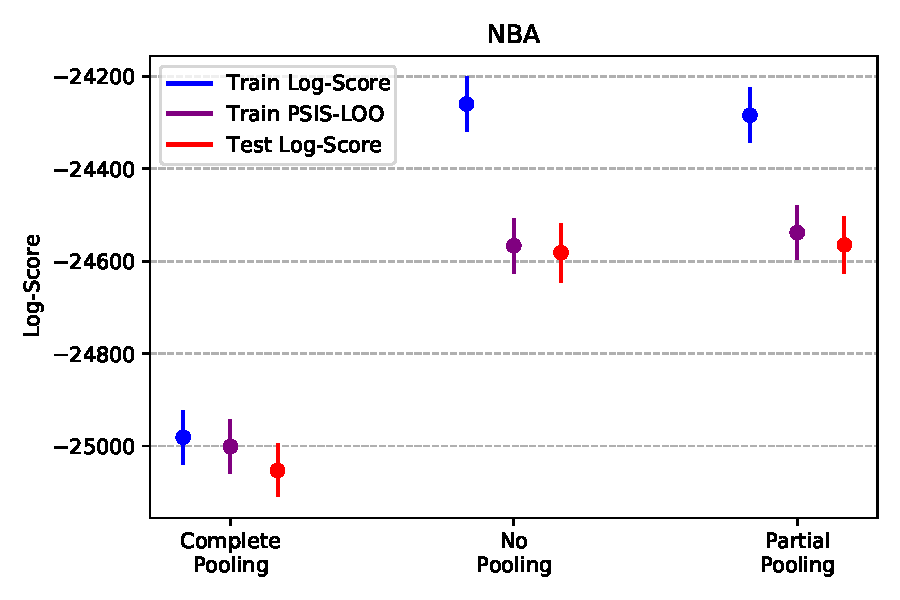
\includegraphics[width=0.5\textwidth]{figures/logscore_NBA.pdf}} \\
	\subfloat[MLB]{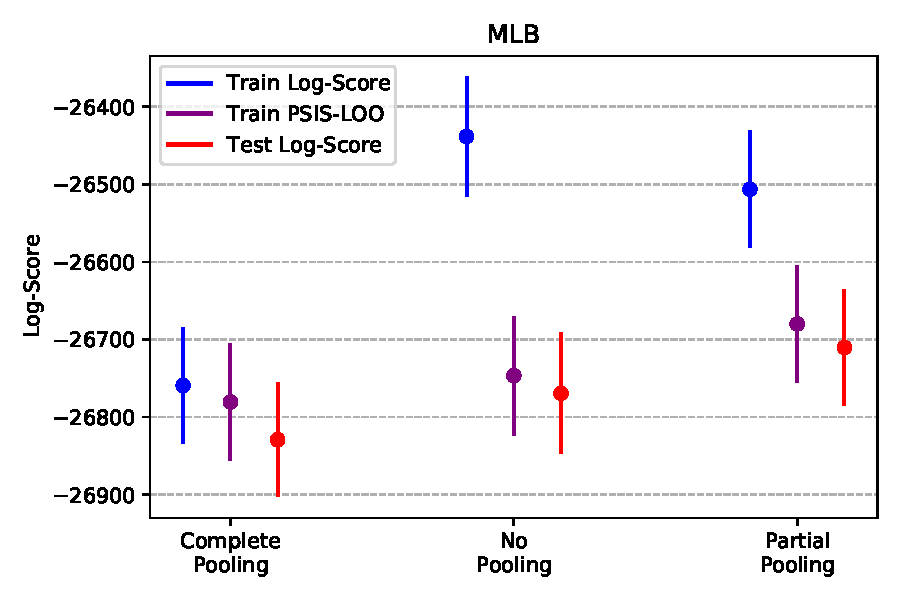
\includegraphics[width=0.5\textwidth]{figures/logscore_MLB.pdf}} 
	\subfloat[NFL]{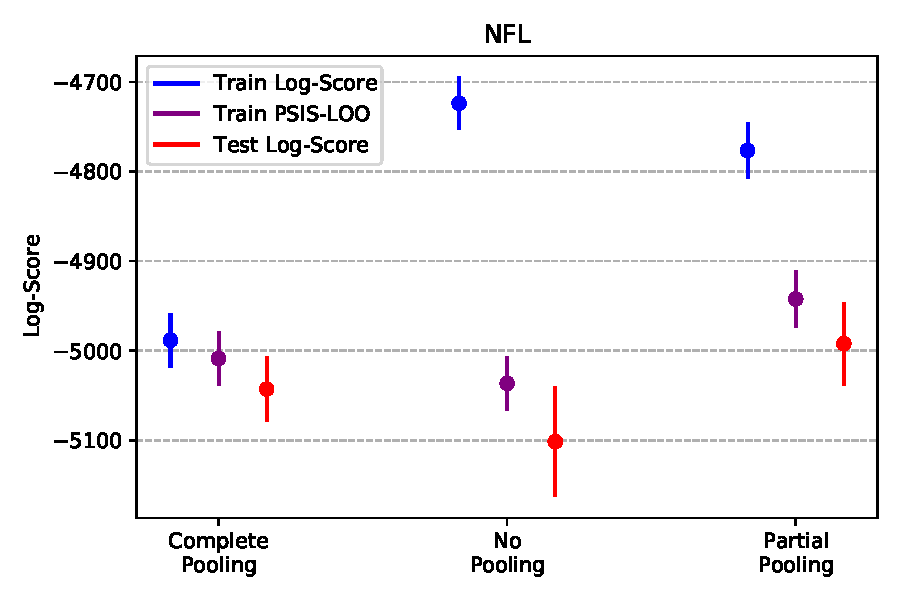
\includegraphics[width=0.5\textwidth]{figures/logscore_NFL.pdf}}
	\caption{Comparison of models via their Log-Score on train and test sets, as well as the PSIS-LOO estimated Log-Score, for each league. The complete-pooling model underfits, the no-pooling model overfits, and the partial-pooling model provides the best tradeoff in fitting the data while protecting against overfitting. The PSIS-LOO estimates consistently predict how the models would rank on an unseen test-set.}
	\label{fig:log_scores}
\end{figure}

\begin{figure}
	\subfloat[NHL]{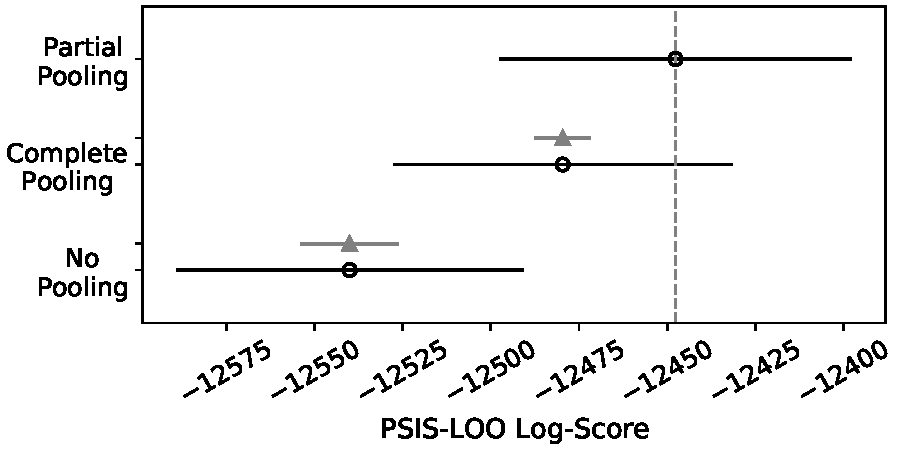
\includegraphics[width=0.5\textwidth]{figures/loo_nhl_no_title.pdf}} 
	\subfloat[NBA]{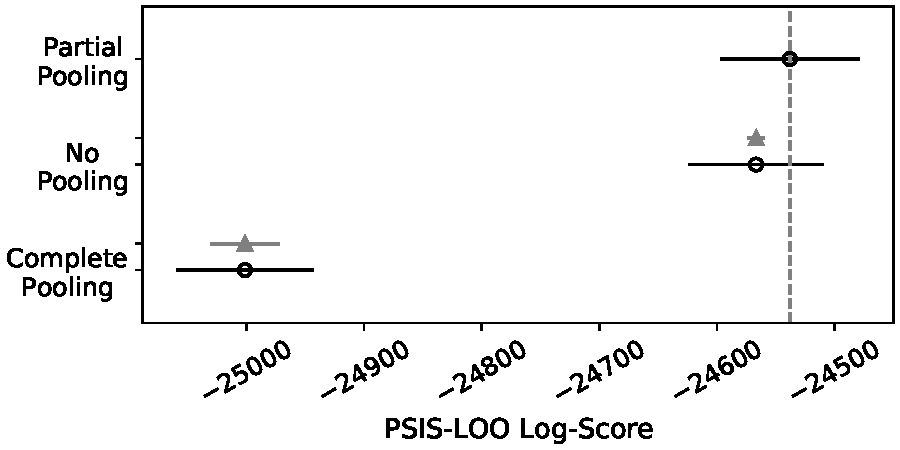
\includegraphics[width=0.5\textwidth]{figures/loo_nba_no_title.pdf}} \\
	\subfloat[MLB]{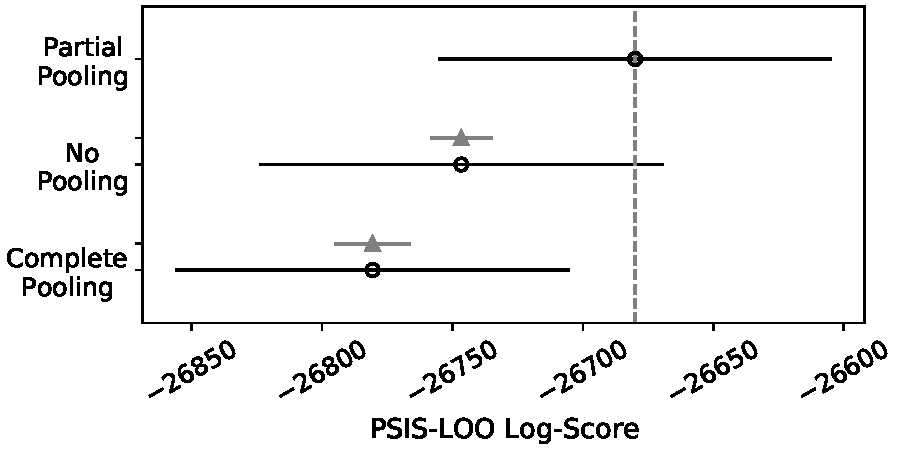
\includegraphics[width=0.5\textwidth]{figures/loo_mlb_no_title.pdf}} 
	\subfloat[NFL]{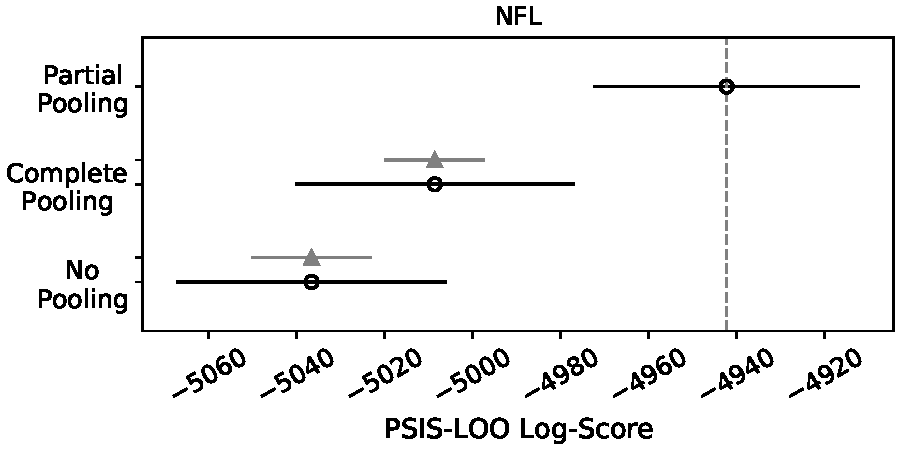
\includegraphics[width=0.5\textwidth]{figures/loo_nfl_no_title.pdf}}
	\caption{Comparison of models via their PSIS-LOO estimated Log-Score for each league, ranked from best (highest) to worst (lowest) on the y-axis. The black points and lines represent the point estimate and its standard error. The grey triangle and lines represent the estimated difference and the standard error of the difference for each model relative to the best model. The standard error of the difference is generally much smaller than the standard error of the estimate because errors in the estimates for each model are highly correlated.}
	\label{fig:psis_loo}
\end{figure}

The results of comparing models via their Log-Score, and how well PSIS-LOO is at estimating the out-of-sample performance, can be seen in Figure \ref{fig:log_scores}. The results show the same general trends across each league: 1) The complete-pooling model underfits the data compared to the other models, but it also overfits less compared to the other models as seen by its test-set performance not degrading as much, 2) The no-pooling model overfits the data the most as it generally has the best performance on the train-set but never has the best performance on the test-set, 3) The partial-pooling model consistently has the best train-set performance and is therefore the best performing model.

These results confirm the advantageous theory behind multilevel modelling explored in chapter ??. The multilevel model (partial-pooling model) consistently outperformed the complete-pooling model on both the train-set and the test-set. Interestingly the multilevel model consistently performed worse than the no-pooling model on the train-set but outperformed the no-pooling model on the test-sets. This is regularization at work and shows the efficacy of multilevel modelling over traditional regression. but fits the train-set worse than the no-pooling model.

The PSIS-LOO estimates of out-of-sample performance consistently ranked the models in the correct order measured by test-set performance, despite only having the train-set available to make these estimates. This shows how effective PSIS-LOO is at estimating out-of-sample performance, why it has become the current state of the art for model evaluation in Bayesian statistics, and why we opt for using PSIS-LOO estimates for ranking models in this thesis. We note that the exact magnitude of the PSIS-LOO estimates were sometimes over or under estimated relative to the test-set results, but that for a given dataset they were consistently over or under estimated. This is interesting because one of the additional contributions of Vehtari et el. (cite) was showing errors in PSIS-LOO estimates are highly correlated for the same dataset. Instead of more naive computations for the standard error, they instead derived an estimated for the standard error of the difference between models trained an evaluated on the same dataset. This new standard error generally provides tighter bounds that more accurately reflect the correlation in errors of PSIS-LOO estimates on the same dataset. A graphical representation of this can be seen in Figure \ref{fig:psis-loos}.

\begin{comment}
\begin{figure}
	\subfloat[NHL]{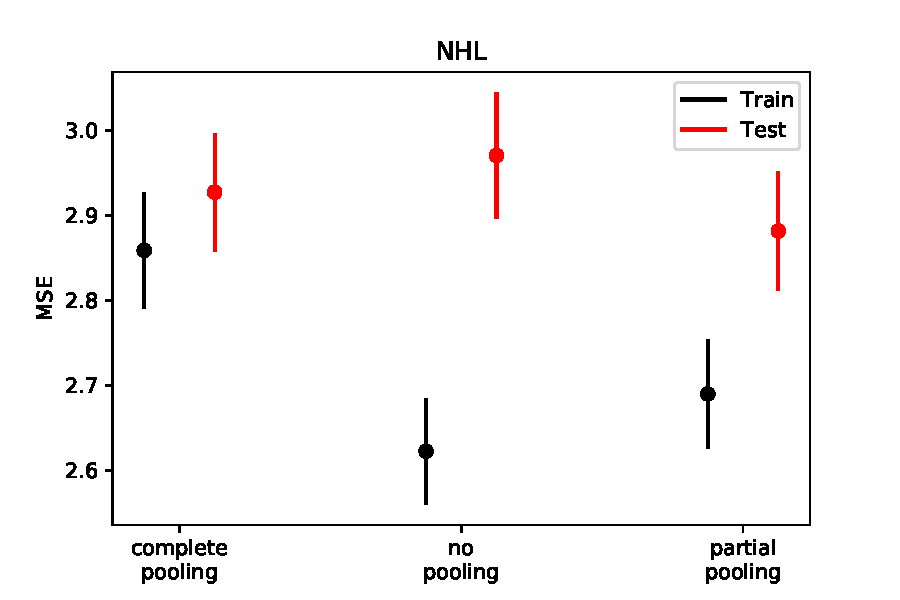
\includegraphics[width=0.5\textwidth]{figures/mse_nhl.pdf}} 
	\subfloat[NBA]{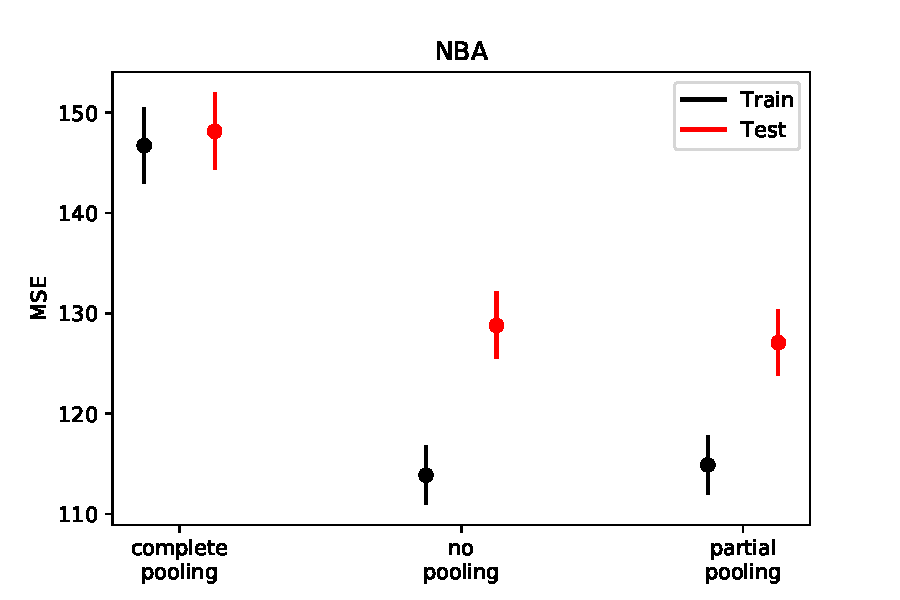
\includegraphics[width=0.5\textwidth]{figures/mse_nba.pdf}} \\
	\subfloat[MLB]{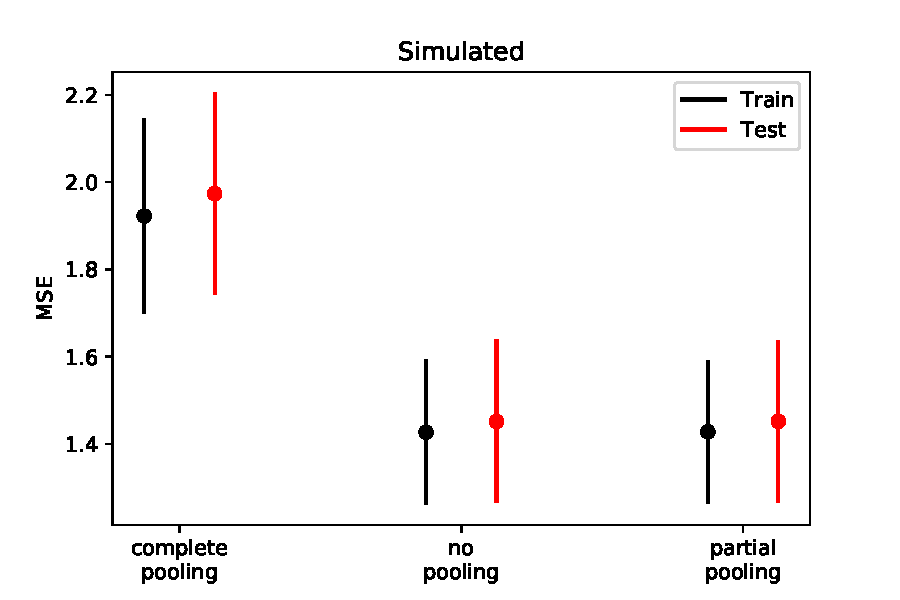
\includegraphics[width=0.5\textwidth]{figures/mse_mlb.pdf}} 
	\subfloat[NFL]{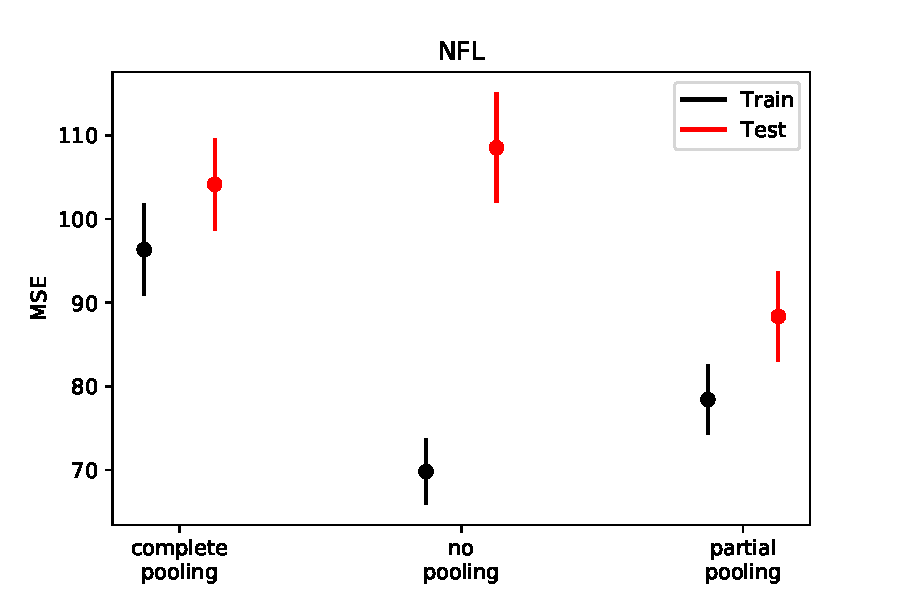
\includegraphics[width=0.5\textwidth]{figures/mse_nfl.pdf}}
	\caption{Comparison of models via their Mean-Squared-Error (MSE) on train and test sets for each league. The complete-pooling model underfits, the no-pooling model overfits, and the partial-pooling model provides the best tradeoff in fitting the data while protecting against overfitting.}
	\label{fig:mses}
\end{figure}

\begin{figure}
	\subfloat[NHL]{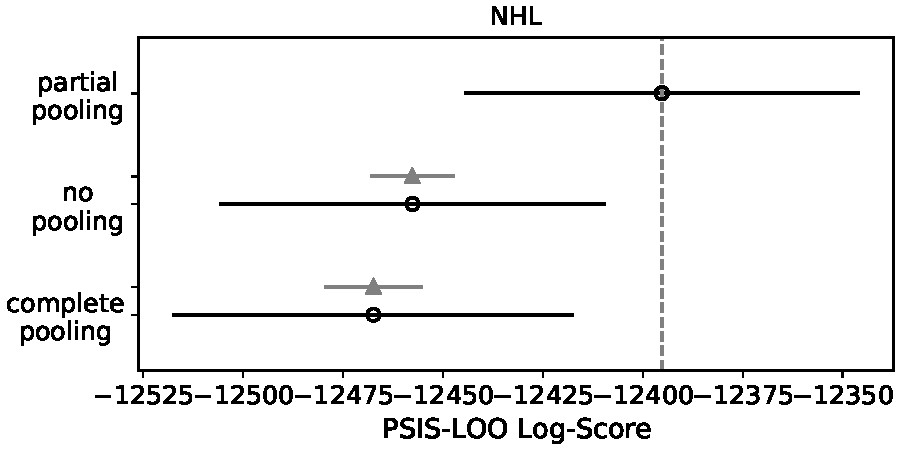
\includegraphics[width=0.5\textwidth]{figures/loo_nhl.pdf}} 
	\subfloat[NBA]{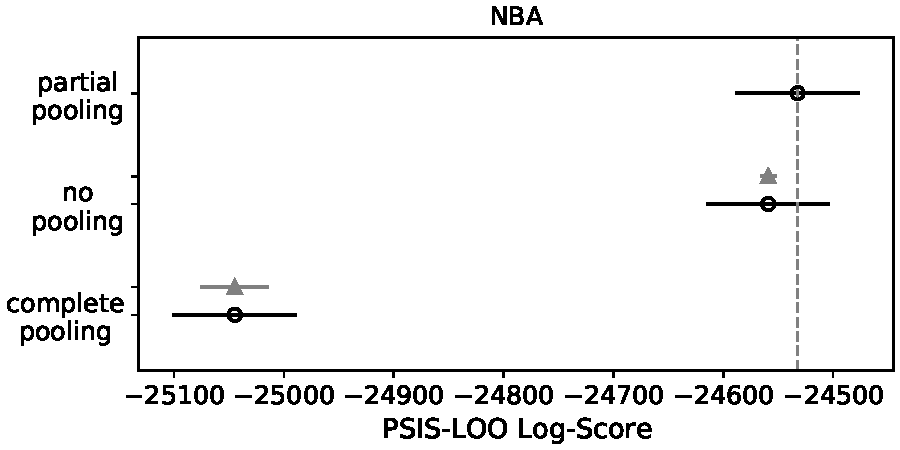
\includegraphics[width=0.5\textwidth]{figures/loo_nba.pdf}} \\
	\subfloat[MLB]{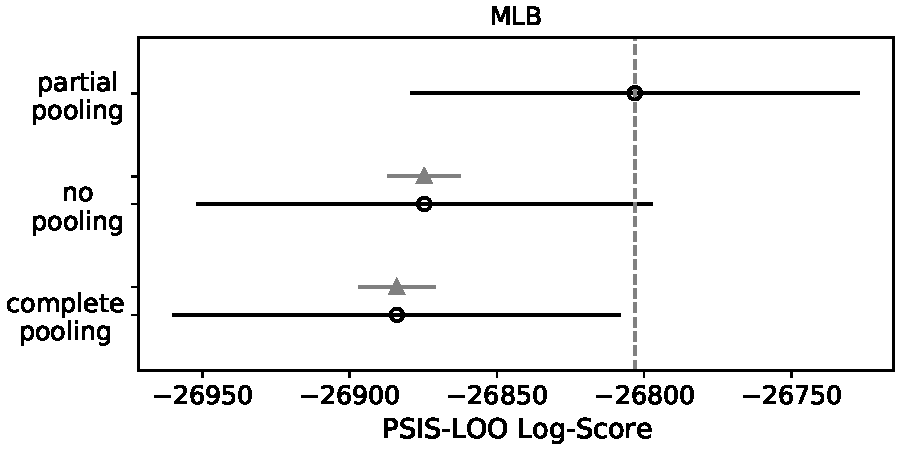
\includegraphics[width=0.5\textwidth]{figures/loo_mlb.pdf}} 
	\subfloat[NFL]{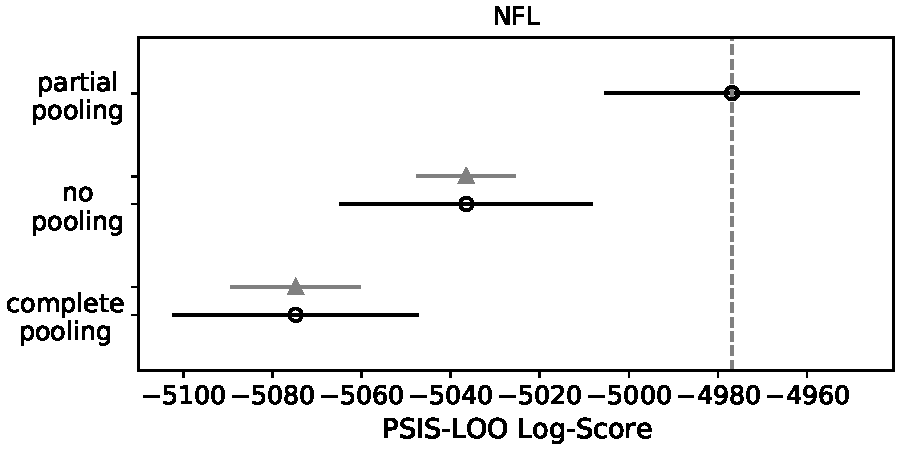
\includegraphics[width=0.5\textwidth]{figures/loo_nfl.pdf}}
	\caption{Comparison of models via their estimated out of sample performance as measured by PSIS-LOO. Since the estimates are computed in the same way on the same data, their errors are highly correlated and the grey error bars represent a more accurate estimate of the standard error of the estimates relative to the best performing model.}
	\label{fig:psis-loos}
\end{figure}
\end{comment}

\subsection{Negative Binomial Regression}

\begin{figure}
	\centering
	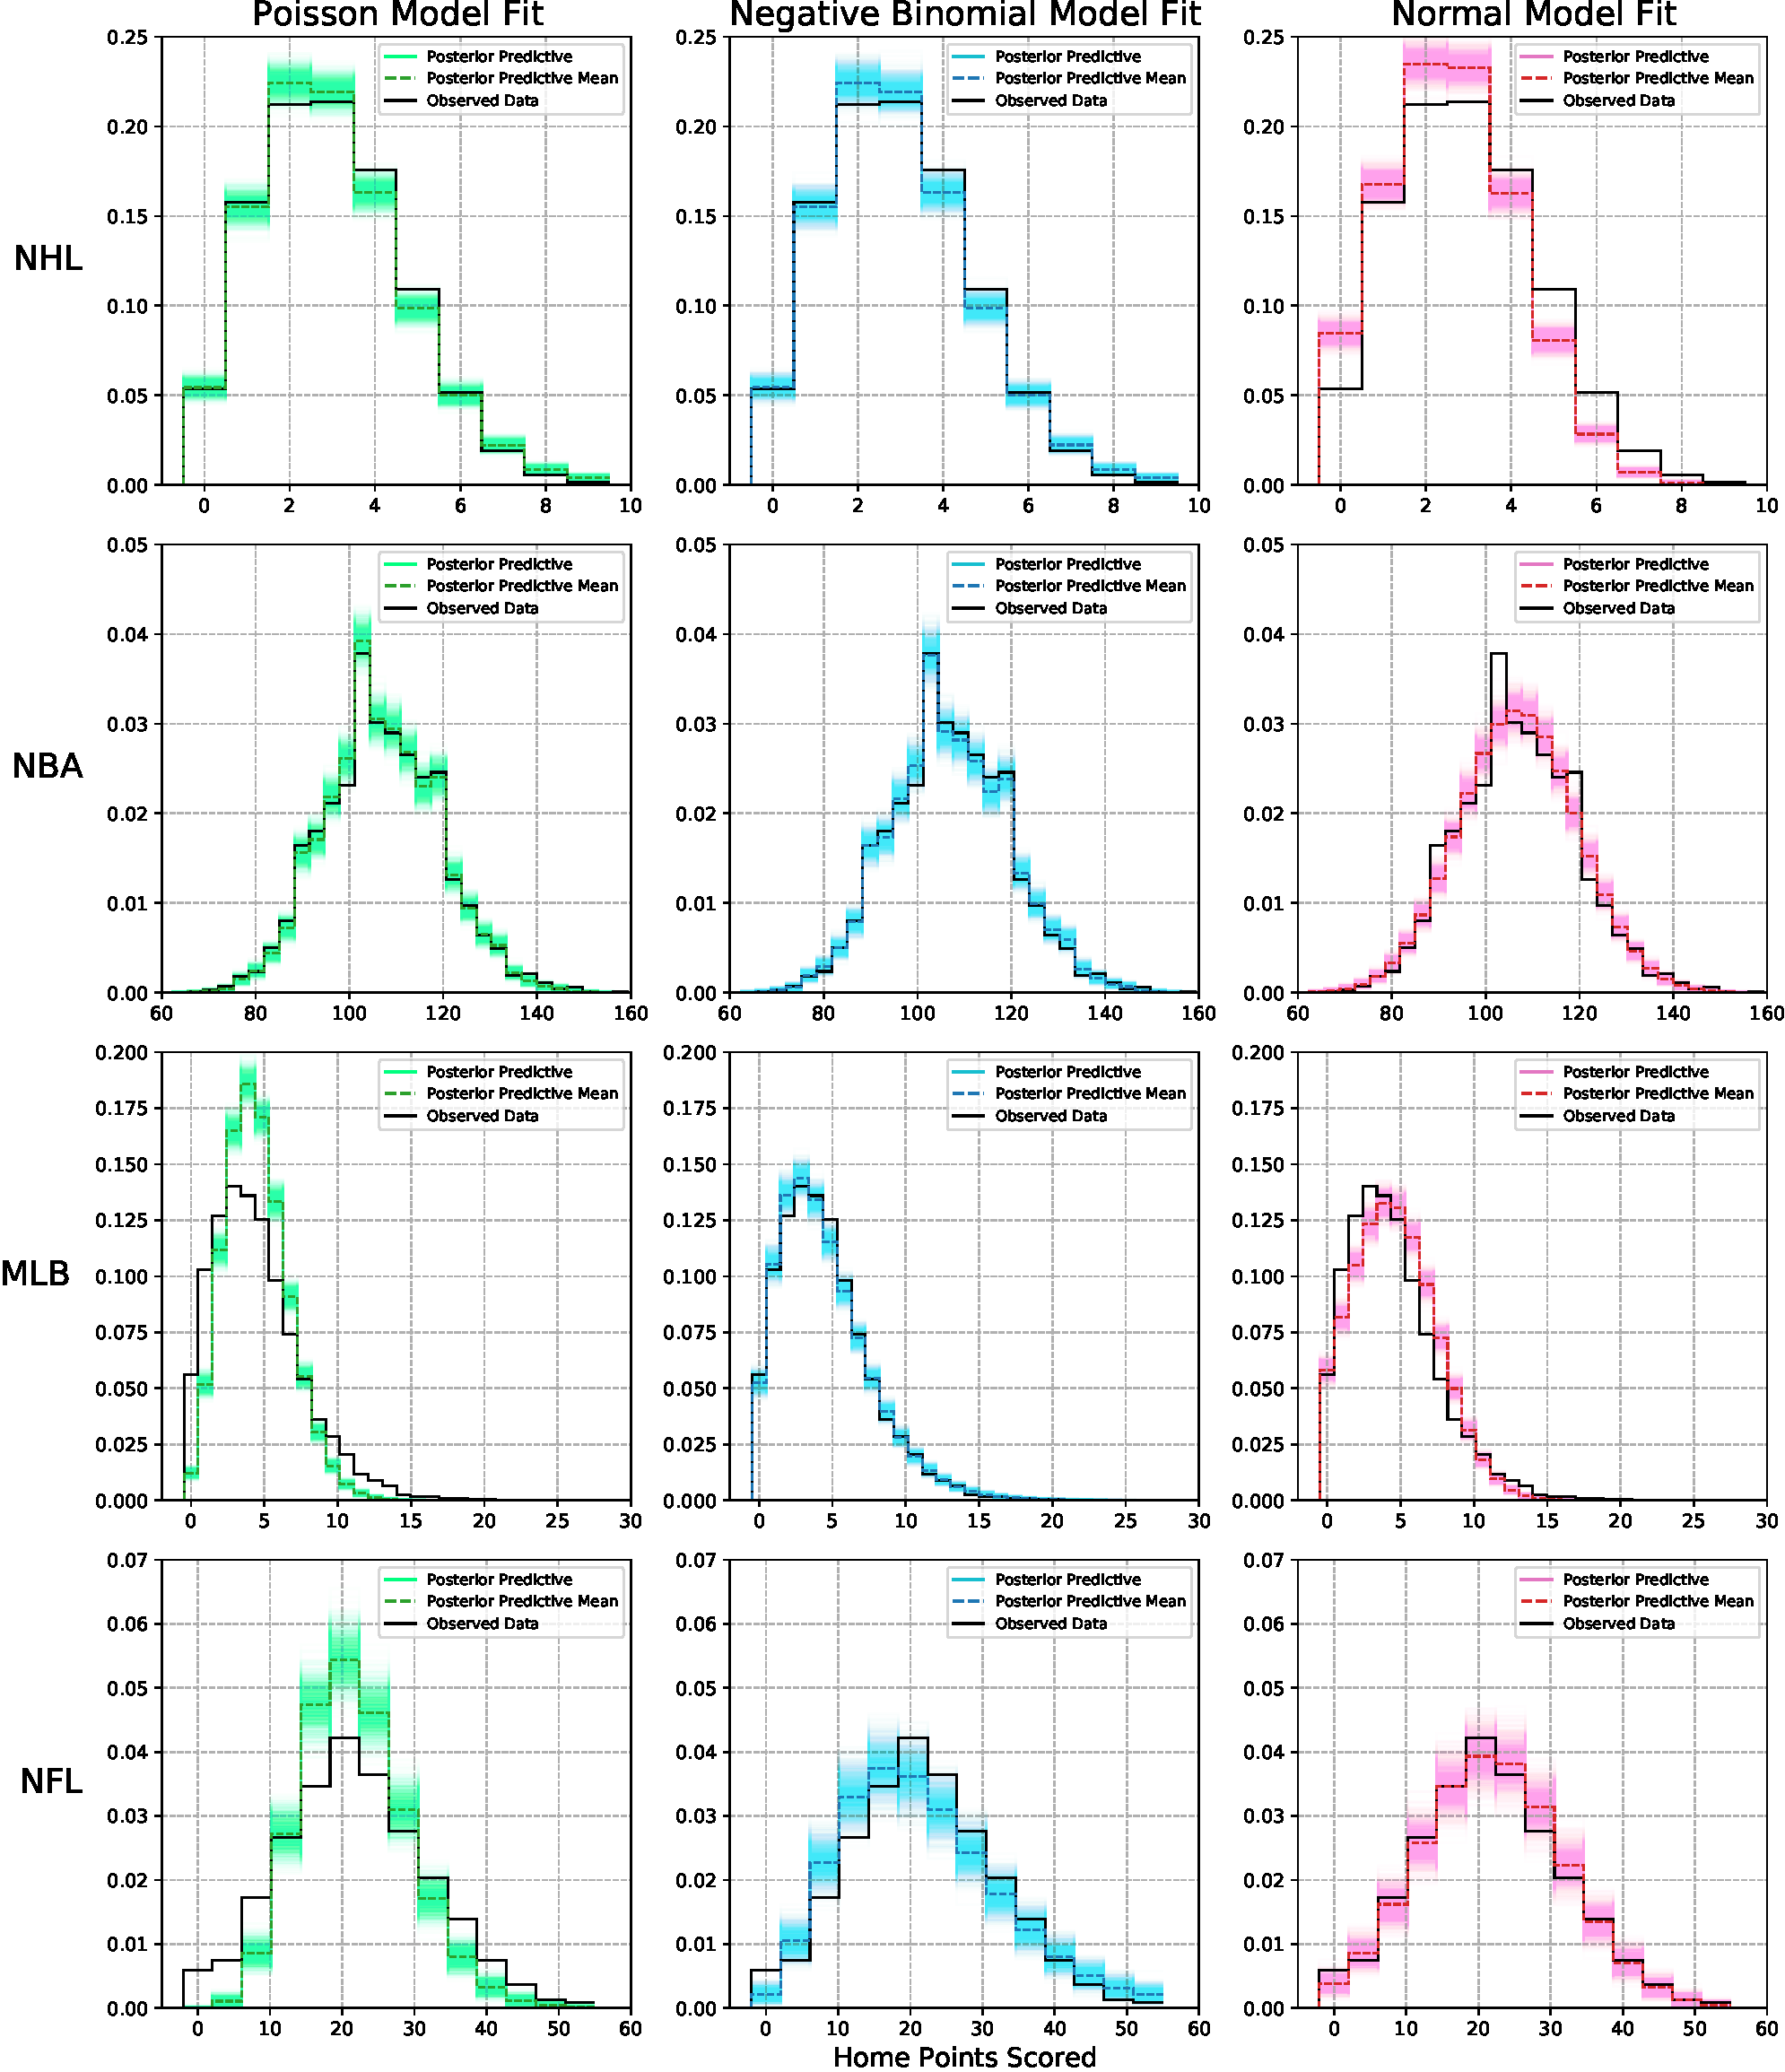
\includegraphics[width=\textwidth]{figures/Figure_3.pdf}
	\caption{Comparison of distribution of home points in the models and the observed data for each league. The Negative Binomial model noticeably provides a better overall fit across each league.}
	\label{fig:comparisons}
\end{figure}

The differences in model fit for the various likelihood distributions considered can be seen visually in Figure \ref{fig:comparisons}. Visually inspecting the distributions in Figure \ref{fig:comparisons} is known as a Posterior Predictive Check (PPC) as described in section ??. The PPCs in Figure \ref{fig:comparisons} are performed by plotting the distribution of observed home point totals in black along with 2000 sampled model fits in green for Poisson, blue for Negative Binomial, and red for Normal; with the respective mean model fits across the 2000 samples as dashed lines. The differences between the Poisson and Negative Binomial models becomes increasingly apparent for the leagues with greater overdispersion, while the Normal model comparatively struggles for each league except the NFL where both the Normal and Negative Binomial greatly outperform the Poisson model. The precise model comparisons are depicted in Table \ref{tab:loo} and reveal the same patterns seen in the models PSIS-LOO estimated out-of-sample predictive fit. Because the point totals of the sports we are considering are positive integers prone to overdispersion and based on the results in Table \ref{tab:loo} and Figure \ref{fig:comparisons}, we conclude that the Negative Binomial distribution is the most appropriate for regression modelling professional hockey, basketball, baseball, and American football.

\begin{table}
\centering
\begin{tabular}{c@{\hskip0.35in}c@{\hskip0.35in}c@{\hskip 0.25in}c@{\hskip 0.25in}c@{\hskip 0.15in}c}
\toprule
& \boldmath$\sigma_p$ & \textbf{Model} & \textbf{PSIS-LOO} & \textbf{dLOO} & \textbf{dSE}\\
\midrule
&& \textbf{Poisson} & \textbf{-24761.3} & - & -\\
NHL & 0.99 & NB & -24761.5 & 0.2 & 0.2\\
&& Normal & -25140.9 & 379.5 & 23.4\\
\midrule
&& Poisson & -49018.3 & 53.5 & 11.0\\
NBA & 1.50 & \textbf{NB} & \textbf{-48964.8} & - & -\\
&& Normal & -48981.9 & 16.6 & 7.5\\
\midrule
&& Poisson & -57458.7 & 4115.8 & 120.9\\
MLB & 2.27 & \textbf{NB} & \textbf{-53342.9} & - & -\\
&& Normal & -55696.8 & 2353.17 & 65.1\\
\midrule
&& Poisson & -11751.2 & 2042.5 & 119.0\\
NFL & 4.56 & NB & -9841.7 & 133.0 & 22.1\\
&& \textbf{Normal} & \textbf{-9708.7} & - & -\\
\bottomrule
\end{tabular}
\caption{Comparison of estimated negative log-likelihood of leave-one-out cross-validation (LOO) for each model across each league. The differences between the Poisson, Negative Binomial (NB), and Normal models are reported relative to the best fitting model (dLOO) for each league; along with the standard error of the estimated differences (dSE). The dispersion statistic, \(\sigma_p\), indicates how much greater the variance is than the mean for point totals in each league and signals overdispersion when \(\sigma_p > 2\). The NB model noticeably outperforms the Poisson model for leagues with greater overdispersion (MLB and NFL) while being nearly identical for leagues with little to no overdispersion (NHL and NBA). The NB model also outperforms the Normal model in each league except the NFL where they are close to one another while both vastly outperforming the Poisson model.}\label{tab:loo}
\end{table}

\subsection{Inferring Home Advantage}

- similar to paper

\begin{figure}
	\centering
	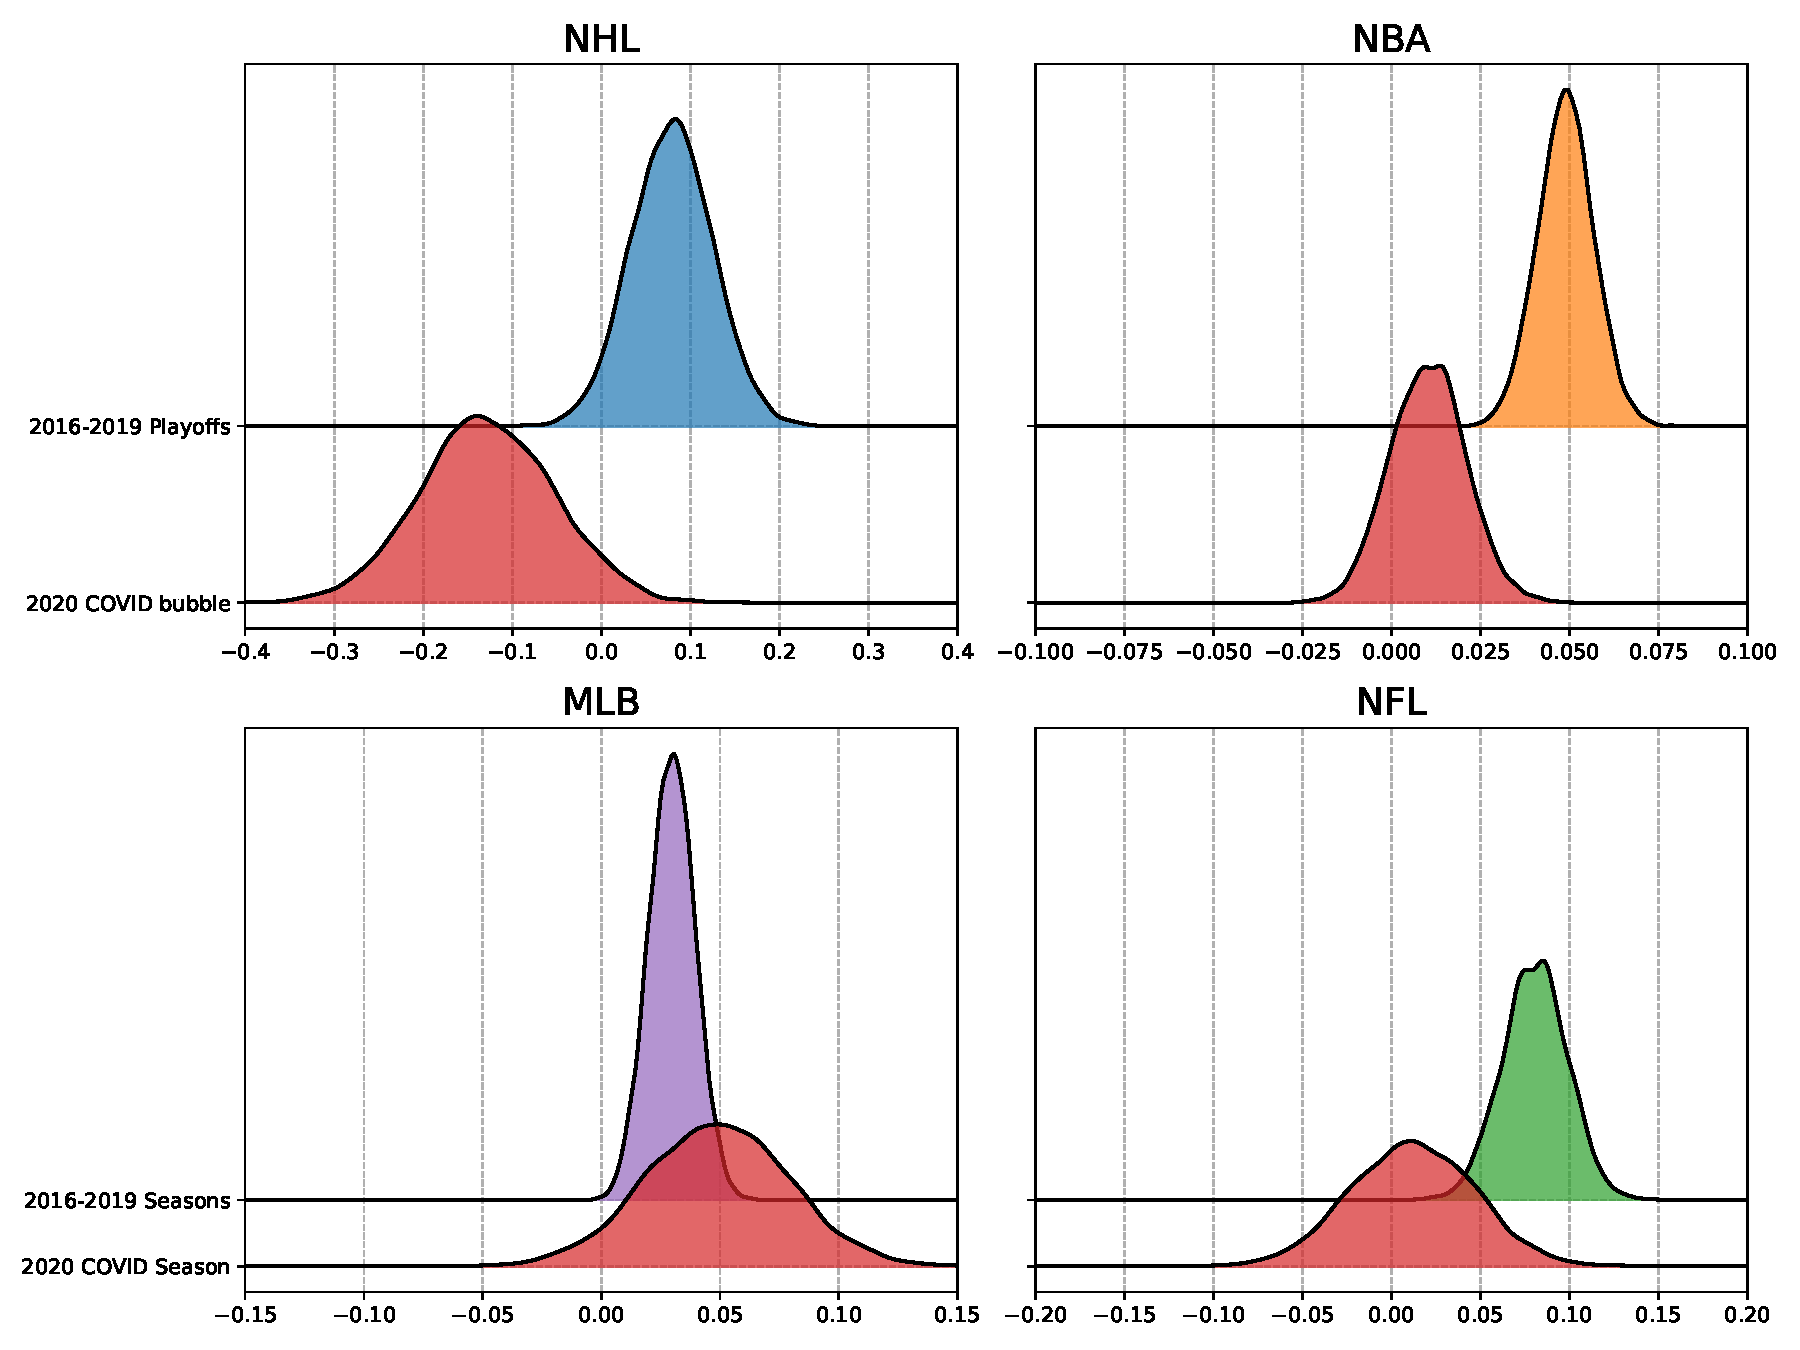
\includegraphics[width=0.9\textwidth]{figures/Figure_1.pdf}
	\caption{Distributions of the estimated home advantage for the NHL, NBA, MLB, and NFL for pre and post COVID adjusted seasons. Home advantage for playoffs are reported for NHL and NBA because that is when their COVID restricted games took place. Home advantage for regular season is reported for MLB and NFL as their respective playoff seasons are too small for stable results. Red distributions represent COVID-19 bubble adjusted seasons.}
	\label{fig:ha_pooled}
\end{figure}

The distributions for the estimates of the home advantage parameters from pooling the previous four pre-COVID-19 seasons/playoffs together can be seen in Figure \mbox{\ref{fig:ha_pooled}} with the COVID-19 restricted season/playoffs coloured red. The peaks of these distributions represent the most likely values for the home advantage parameter and their width represents the uncertainty in these estimates. We can use these distributions to directly measure the probability the home advantage parameter is less than the previous seasons. The leftward shift of the distribution for the COVID-19 restricted season/playoffs suggests that home advantage decreased in the NHL, NBA, and NFL while not changing for the MLB.

Figure \mbox{\ref{fig:ha_main}} shows results from estimating home advantage individually for each prior season. This more granular view of pre-COVID-19 home advantage reveals greater season-to-season variation in home advantage that is missing in Figure \mbox{\ref{fig:ha_pooled}}. Nevertheless, the year-over-year estimates in Figure \mbox{\ref{fig:ha_main}} show the results of reduced home advantage in COVID-19 restricted season/playoffs holding for the NHL, NFL, and NBA, albeit with a single past season with lower home advantage in both the NFL and NBA. The remainder of this section examines these estimated distributions and their implications.

For the NHL and NBA data, Figures \mbox{\ref{fig:ha_pooled}} and \mbox{\ref{fig:ha_main}} and our analysis focus on their playoff seasons because the NHL and NBA COVID-19 seasons only took place during their playoff seasons. In contrast, the MLB and NFL had COVID-19 restrictions for their entire seasons, therefore, Figures \mbox{\ref{fig:ha_pooled}} and \mbox{\ref{fig:ha_main}}, and our analysis for those leagues are focused on their regular season games. Focusing on the MLB and NFL regular seasons is not only convenient but arguably necessary as their playoff seasons consist of much fewer games than the NHL and NBA playoff seasons, resulting in high uncertainty of parameter estimates. The NHL and NBA regular season results as well as the MLB and NFL playoff results are provided in the supplementary materials.

The home advantage parameter, $\beta$, represents a multiplier of $\text{exp}(\beta)$ applied to expected points. For example, an estimated home advantage parameter for the NBA of $0.05$ represents a $\text{exp}(0.05) \approx 1.0513$ multiplier on expected points or an increase in expected points of 5\%. With average points scored in the NBA being around 107 this would translate to approximately a 5-point home advantage on average in the NBA playoffs. We provide a full description and interpretation of the model in the Methods section.

For the NHL data, the results in both Figures \mbox{\ref{fig:ha_pooled}} and \mbox{\ref{fig:ha_main}} show the home advantage parameter confidently above 0 for pre-COVID-19 seasons and confidently below 0 for the COVID-19 bubble. The probability the home advantage parameter $(\beta)$ is less than 0 for the COVID-19 bubble is $\Pr(\beta < 0) = 0.95$. The probability the home advantage parameter is less than the previous playoff seasons mean of $0.081$ is $0.998$. These results give strong evidence that home advantage in the NHL was negatively impacted by the COVID-19 bubble.

For the NBA data, the pooled home advantage parameter estimate in Figure \mbox{\ref{fig:ha_pooled}} is confidently above 0 and tightly around 0.05. For the COVID-19 affected playoffs, the probability the home advantage is less than 0 is only $0.17$, but the probability that it is less than the pre-COVID-19 mean of 0.05 is $0.999$, suggesting that home advantage in the NBA was negatively impacted by the COVID-19 bubble. However, when examining the year-to-year estimates of prior seasons in Figure \mbox{\ref{fig:ha_main}} we see a decreasing trend in home advantage in the NBA playoffs with the estimate for the NBA playoffs in 2017 appearing as almost as much of an outlier as the COVID-19 estimate. This suggests the decreased home advantage in the COVID-19 could potentially be a random outlier. The uncertainty in these estimates means we can not make definitive conclusions in the absence of more data. We conclude that it is probable that home advantage in the NBA decreased in the COVID-19 bubble but not as definitively as the NHL results.

For the MLB data, the home advantage parameter is surprisingly likely to be slightly greater than it had been in previous seasons. The probability the home advantage parameter is less than the mean of the previous seasons is $\Pr(\beta < 0.036) = 0.26$. When comparing the COVID-19 estimate to the previous seasons in Figure \mbox{\ref{fig:ha_main}} there appears to be no noteworthy difference. This gives evidence that home advantage in the MLB was unlikely to be negatively impacted by the COVID-19 restrictions and was likely unaffected by the restrictions.

For the NFL data, the pooled home advantage parameter estimate in Figure \mbox{\ref{fig:ha_pooled}} is confidently above 0 with a mean of 0.078. For the COVID-19 affected season, the probability the home advantage is less than 0 is $0.388$, but the probability that it is less than the pre-COVID-19 mean of 0.078 is $0.976$, suggesting that home advantage in the NFL was negatively impacted by the COVID-19 restrictions. However, when examining the year-to-year estimates of prior seasons there is a clear pattern of home advantage decreasing in the NFL and even being lower in 2019 than it was in the 2020 COVID-19 adjusted season. We argue the results in Figure \mbox{\ref{fig:ha_main}} are enough to overturn the results in Figure \mbox{\ref{fig:ha_pooled}} and conclude that home advantage in the NFL was not impacted from its previous trend by the COVID-19 restrictions.

In summary, results for pooled (Figure~\mbox{\ref{fig:ha_pooled}}) and individual~(Figure~\mbox{\ref{fig:ha_main}}) past seasons give strong evidence that home advantage in the NHL was negatively impacted during the COVID-19 restricted playoff season and that home advantage in the MLB was unaffected by the restrictions. Pooled past season results also suggest home advantage was negatively impacted by the COVID-19 restricted seasons for the NBA and NFL, however a closer examination of the individual past season results reveals a trend of decreasing home advantage over the past few seasons, which may partly account for the lower home advantage found during NBA and NFL COVID-19 restrictions.

\begin{figure}
	\centering
	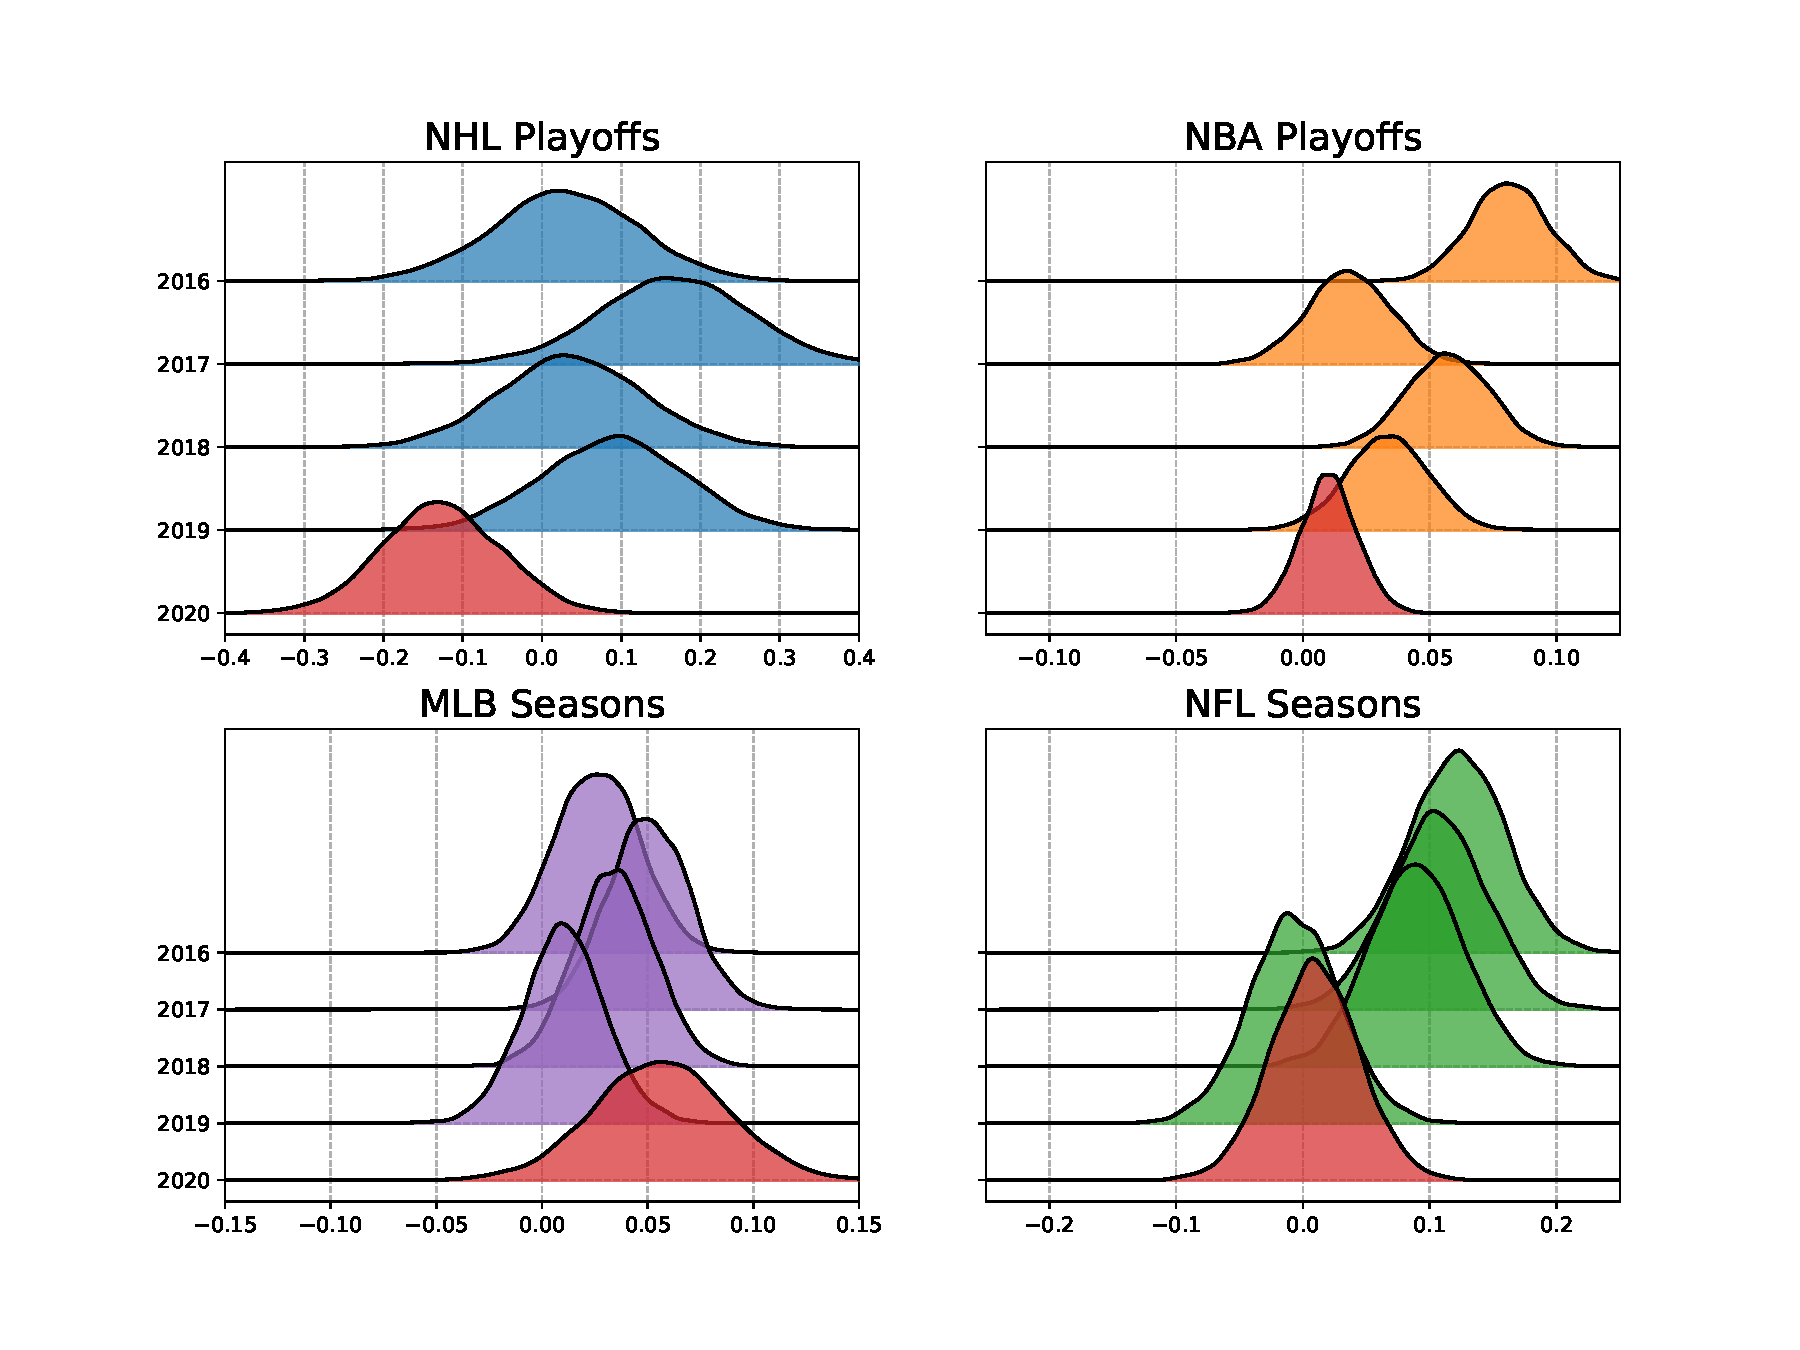
\includegraphics[width=\textwidth]{figures/Figure_2.pdf}
	\caption{Distributions of the estimated home advantage for the NHL, NBA, MLB, and NFL over the past 5 seasons from 2016-2020. Home advantage for playoffs are reported for NHL and NBA because that is when their COVID restricted games took place. Home advantage for regular season is reported for MLB and NFL as their respective playoff seasons are too small for stable results. Red distributions represent COVID-19 bubble adjusted seasons.}
	\label{fig:ha_main}
\end{figure}